% Options for packages loaded elsewhere
\PassOptionsToPackage{unicode}{hyperref}
\PassOptionsToPackage{hyphens}{url}
%
\documentclass[
  english,
  man,floatsintext]{apa6}
\usepackage{lmodern}
\usepackage{amssymb,amsmath}
\usepackage{ifxetex,ifluatex}
\ifnum 0\ifxetex 1\fi\ifluatex 1\fi=0 % if pdftex
  \usepackage[T1]{fontenc}
  \usepackage[utf8]{inputenc}
  \usepackage{textcomp} % provide euro and other symbols
\else % if luatex or xetex
  \usepackage{unicode-math}
  \defaultfontfeatures{Scale=MatchLowercase}
  \defaultfontfeatures[\rmfamily]{Ligatures=TeX,Scale=1}
\fi
% Use upquote if available, for straight quotes in verbatim environments
\IfFileExists{upquote.sty}{\usepackage{upquote}}{}
\IfFileExists{microtype.sty}{% use microtype if available
  \usepackage[]{microtype}
  \UseMicrotypeSet[protrusion]{basicmath} % disable protrusion for tt fonts
}{}
\makeatletter
\@ifundefined{KOMAClassName}{% if non-KOMA class
  \IfFileExists{parskip.sty}{%
    \usepackage{parskip}
  }{% else
    \setlength{\parindent}{0pt}
    \setlength{\parskip}{6pt plus 2pt minus 1pt}}
}{% if KOMA class
  \KOMAoptions{parskip=half}}
\makeatother
\usepackage{xcolor}
\IfFileExists{xurl.sty}{\usepackage{xurl}}{} % add URL line breaks if available
\IfFileExists{bookmark.sty}{\usepackage{bookmark}}{\usepackage{hyperref}}
\hypersetup{
  pdftitle={Associations between cognitive and affective empathy and internalizing symptoms in late childhood},
  pdflang={en-EN},
  pdfkeywords={keywords},
  hidelinks,
  pdfcreator={LaTeX via pandoc}}
\urlstyle{same} % disable monospaced font for URLs
\usepackage{graphicx,grffile}
\makeatletter
\def\maxwidth{\ifdim\Gin@nat@width>\linewidth\linewidth\else\Gin@nat@width\fi}
\def\maxheight{\ifdim\Gin@nat@height>\textheight\textheight\else\Gin@nat@height\fi}
\makeatother
% Scale images if necessary, so that they will not overflow the page
% margins by default, and it is still possible to overwrite the defaults
% using explicit options in \includegraphics[width, height, ...]{}
\setkeys{Gin}{width=\maxwidth,height=\maxheight,keepaspectratio}
% Set default figure placement to htbp
\makeatletter
\def\fps@figure{htbp}
\makeatother
\setlength{\emergencystretch}{3em} % prevent overfull lines
\providecommand{\tightlist}{%
  \setlength{\itemsep}{0pt}\setlength{\parskip}{0pt}}
\setcounter{secnumdepth}{-\maxdimen} % remove section numbering
% Make \paragraph and \subparagraph free-standing
\ifx\paragraph\undefined\else
  \let\oldparagraph\paragraph
  \renewcommand{\paragraph}[1]{\oldparagraph{#1}\mbox{}}
\fi
\ifx\subparagraph\undefined\else
  \let\oldsubparagraph\subparagraph
  \renewcommand{\subparagraph}[1]{\oldsubparagraph{#1}\mbox{}}
\fi
% Manuscript styling
\usepackage{upgreek}
\captionsetup{font=singlespacing,justification=justified}

% Table formatting
\usepackage{longtable}
\usepackage{lscape}
% \usepackage[counterclockwise]{rotating}   % Landscape page setup for large tables
\usepackage{multirow}		% Table styling
\usepackage{tabularx}		% Control Column width
\usepackage[flushleft]{threeparttable}	% Allows for three part tables with a specified notes section
\usepackage{threeparttablex}            % Lets threeparttable work with longtable

% Create new environments so endfloat can handle them
% \newenvironment{ltable}
%   {\begin{landscape}\begin{center}\begin{threeparttable}}
%   {\end{threeparttable}\end{center}\end{landscape}}
\newenvironment{lltable}{\begin{landscape}\begin{center}\begin{ThreePartTable}}{\end{ThreePartTable}\end{center}\end{landscape}}

% Enables adjusting longtable caption width to table width
% Solution found at http://golatex.de/longtable-mit-caption-so-breit-wie-die-tabelle-t15767.html
\makeatletter
\newcommand\LastLTentrywidth{1em}
\newlength\longtablewidth
\setlength{\longtablewidth}{1in}
\newcommand{\getlongtablewidth}{\begingroup \ifcsname LT@\roman{LT@tables}\endcsname \global\longtablewidth=0pt \renewcommand{\LT@entry}[2]{\global\advance\longtablewidth by ##2\relax\gdef\LastLTentrywidth{##2}}\@nameuse{LT@\roman{LT@tables}} \fi \endgroup}

% \setlength{\parindent}{0.5in}
% \setlength{\parskip}{0pt plus 0pt minus 0pt}

% \usepackage{etoolbox}
\makeatletter
\patchcmd{\HyOrg@maketitle}
  {\section{\normalfont\normalsize\abstractname}}
  {\section*{\normalfont\normalsize\abstractname}}
  {}{\typeout{Failed to patch abstract.}}
\makeatother
\shorttitle{Empathy and internalizing symptoms in late childhood}
\author{Katherine O. Bray\textsuperscript{1,2}, Vicki Anderson\textsuperscript{2,3}, Christos Pantelis\textsuperscript{1}, Elena Pozzi\textsuperscript{1,4}, Orli S. Schwartz\textsuperscript{4}, Nandita Vijayakumar\textsuperscript{5}, Sally Richmond\textsuperscript{6}, Camille Deane\textsuperscript{5}, Nicholas B. Allen\textsuperscript{7}, \& Sarah Whittle\textsuperscript{1}}
\affiliation{
\vspace{0.5cm}
\textsuperscript{1} Melbourne Neuropsychiatry Centre (MNC), Department of Psychiatry, The University of Melbourne \& Melbourne Health, Melbourne, Australia\\\textsuperscript{2} Melbourne School of Psychological Sciences, University of Melbourne, Melbourne, Australia\\\textsuperscript{3} Murdoch Children's Research Centre, Melbourne, Australia\\\textsuperscript{4} Orygen, Melbourne Australia, Centre for Youth Mental Health, University of Melbourne, Australia\\\textsuperscript{5} School of Psychology, Deakin University, Melbourne, Australia\\\textsuperscript{6} Turner Institute for Brain and Mental Health, School of Psychological Sciences, Monash University, Melbourne, Australia\\\textsuperscript{7} Department of Psychology, University of Oregon, USA}
\authornote{Add complete departmental affiliations for each author here. Each new line herein must be indented, 
like this line.

Enter author note here.


Correspondence concerning this article should be addressed to Katherine O. Bray, Postal address. E-mail: my@email.com}
\keywords{keywords\newline\indent Word count: X}
\usepackage{lineno}

\linenumbers
\usepackage{csquotes}
\ifxetex
  % Load polyglossia as late as possible: uses bidi with RTL langages (e.g. Hebrew, Arabic)
  \usepackage{polyglossia}
  \setmainlanguage[]{english}
\else
  \usepackage[shorthands=off,main=english]{babel}
\fi

\title{Associations between cognitive and affective empathy and internalizing symptoms in late childhood}

\date{}

\abstract{
Empathy is a multidimensional construct, which includes cognitive (i.e., understanding another's
emotional state) and affective (i.e., experiencing and reacting to another's emotional state)
components. Studies in adults have demonstrated that both affective and cognitive empathy are
related to anxious and depressive symptoms. The aim of this study was to examine these associations
in childhood, where there is relatively less research. Participants were 127 9- and 10-year-old
children, recruited from the community. Self-report measures of cognitive and affective empathy,
and internalizing symptoms were administered, as well as a task-based measure of cognitive empathy.
Canonical correlation analysis demonstrated that components of affective empathy, specifically
affective sharing and empathic distress, were associated with internalizing (particularly social
anxiety) symptoms. Although empathy is important for successful social interaction, this study
suggests that children who share each other's emotions strongly are more likely to experience
anxiety, particularly of a social nature.
}

\begin{document}
\maketitle

\hypertarget{data-analysis}{%
\subsection{Data analysis}\label{data-analysis}}

\#We used R (Version 4.0.2; R Core Team, 2020) and the R-packages \emph{AMR} (Version 1.2.0; Berends et al., 2019), \emph{apaTables} (Version 2.0.5; Stanley, 2018), \emph{car} (Version 3.0.8; Fox \& Weisberg, 2019; Fox, Weisberg, \& Price, 2020), \emph{carData} (Version 3.0.4; Fox et al., 2020), \emph{corrplot2017} (Wei \& Simko, 2017), \emph{corx} (Version 1.0.6.1; Conigrave, 2020), \emph{dplyr} (Version 1.0.0; Wickham, François, Henry, \& Müller, 2020), \emph{GGally} (Version 2.0.0; Schloerke et al., 2020), \emph{ggplot2} (Version 3.3.2; Wickham, 2016), \emph{gridExtra} (Version 2.3; Auguie, 2017), \emph{jtools} (Version 2.1.0; Long, 2020), \emph{lubridate} (Version 1.7.9; Grolemund \& Wickham, 2011), \emph{MASS} (Version 7.3.51.6; Venables \& Ripley, 2002), \emph{mctest} (Version 1.3; Imdadullah, Aslam, \& Altaf, 2016; Imdad, Aslam, Altaf, \& Munir, 2019), \emph{numform} (Version 0.6.0; Rinker, 2020), \emph{papaja} (Version 0.1.0.9942; Aust \& Barth, 2020), \emph{plyr} (Version 1.8.6; Wickham et al., 2020; Wickham, 2011), \emph{ppcor} (Version 1.1; Kim, 2015), and \emph{psych} (Version 1.9.12.31; Revelle, 2019) for all our analyses.

\hypertarget{results}{%
\section{Results}\label{results}}

\hypertarget{canonical-correlation-analysis}{%
\subsection{Canonical Correlation Analysis}\label{canonical-correlation-analysis}}

\begin{center}
\begin{ThreePartTable}

\begin{TableNotes}[para]
\normalsize{\textit{Note.} Est. FSIQ = Estimated full scale IQ, Neighborhood advantage is listed from least 
  advantage to most}
\end{TableNotes}

\small{

\begin{longtable}{lcc}\noalign{\getlongtablewidth\global\LTcapwidth=\longtablewidth}
\caption{\label{tab:desctable}Descriptive statistics characterizing the sample used for the CCA analysis}\\
\toprule
Demographic measure & Frequency or Mean & Percentage or Stnd. Dev.\\
\midrule
\endfirsthead
\caption*{\normalfont{Table \ref{tab:desctable} continued}}\\
\toprule
Demographic measure & Frequency or Mean & Percentage or Stnd. Dev.\\
\midrule
\endhead
Sex &  & \\
\ \ \ Female & 68 & 53.54\\
\ \ \ Male & 59 & 46.46\\
Age &  & \\
\ \ \ blank1 & 10 & 4.55\\
Est. FSIQ &  & \\
\ \ \ blank2 & 106 & 10.91\\
Parent Education &  & \\
\ \ \ Grade 7 to 12 & 13 & 10.24\\
\ \ \ Graduated High School & 10 & 7.87\\
\ \ \ Partial tertiary university & 5 & 3.94\\
\ \ \ TAFE & 21 & 16.54\\
\ \ \ Bachelor’s degree & 29 & 22.83\\
\ \ \ Honors & 4 & 3.15\\
\ \ \ Partial graduate school & 9 & 7.09\\
\ \ \ Completed graduate school & 36 & 28.35\\
Neighborhood advantage &  & \\
\ \ \ Quintile 1 & 28 & 22.05\\
\ \ \ Quintile 2 & 33 & 25.98\\
\ \ \ Quintile 3 & 30 & 23.62\\
\ \ \ Quintile 4 & 24 & 18.90\\
\ \ \ Quintile 5 & 12 & 9.45\\
Race &  & \\
\ \ \ White & 92 & 72.44\\
\ \ \ Asian & 14 & 11.02\\
\ \ \ Mixed or other & 14 & 11.02\\
\ \ \ Missing & 7 & 5.51\\
Ethnicity &  & \\
\ \ \ Australian 
\ \ \ \ \ \ \ \ \ \ \ \ \ \ \ \ \ \ \ \ \ \ \ \ \ \ (or New Zealander) & 75 & 59.06\\
\ \ \ Australian/European & 17 & 13.39\\
\ \ \ Australian/Asian & 11 & 8.66\\
\ \ \ Asian1 & 6 & 4.72\\
\ \ \ European & 3 & 2.36\\
\ \ \ Other & 8 & 6.30\\
\ \ \ Missin & 7 & 5.51\\
\bottomrule
\addlinespace
\insertTableNotes
\end{longtable}

}

\end{ThreePartTable}
\end{center}

\begin{table}[tbp]

\begin{center}
\begin{threeparttable}

\caption{\label{tab:meanstable}Means, standard deviations, range, skew and kurtosis for the key measures 
  used in the CCA}

\small{

\begin{tabular}{lccccccc}
\toprule
Measure of interest & $N$ & Mean & $SD$ & Range & Skew & Kurtosis & Cronbach’s $\alpha$\\
\midrule
Empathy &  &  &  &  &  &  & \\
\ \ \ Affective Sharing & 127 & 9.59 & 3.69 & 16.00 & 0.35 & -0.22 & .84\\
\ \ \ Cognitive Empathy & 127 & 13.34 & 2.79 & 16.00 & -0.15 & 0.06 & .68\\
\ \ \ Empathic Concern & 127 & 16.53 & 2.32 & 11.00 & -0.43 & -0.17 & .58\\
\ \ \ Empathic Distress & 127 & 8.16 & 3.09 & 15.00 & 0.31 & -0.29 & .64\\
\ \ \ Silent Films & 127 & 7.68 & 2.21 & 11.00 & -0.54 & 0.44 & .31\\
CDI (before binarization) &  &  &  &  &  &  & \\
\ \ \ Neg. mood/phys. symptoms & 127 & 2.61 & 2.31 & 9.00 & 0.68 & -0.42 & .62\\
\ \ \ Negative self-esteem & 127 & 0.84 & 1.20 & 5.00 & 1.62 & 2.07 & .61\\
\ \ \ Ineffectiveness & 127 & 2.63 & 2.43 & 10.00 & 0.95 & 0.06 & .70\\
\ \ \ Interpersonal problems & 127 & 0.73 & 1.21 & 5.00 & 1.70 & 1.91 & .65\\
SCAS &  &  &  &  &  &  & \\
\ \ \ Separation anxiety & 127 & 3.96 & 3.03 & 16.00 & 0.96 & 1.23 & .71\\
\ \ \ Social phobia & 127 & 3.51 & 2.91 & 12.00 & 0.77 & -0.14 & .75\\
\ \ \ Physical injury fears & 127 & 3.65 & 2.59 & 12.00 & 0.72 & 0.15 & .75\\
\ \ \ Generalized anxiety & 127 & 4.94 & 2.94 & 16.00 & 0.65 & 0.52 & .74\\
\ \ \ Obsessive compulsive & 127 & 5.02 & 3.42 & 14.00 & 0.53 & -0.21 & .52\\
\ \ \ Panic/agoraphobia & 127 & 2.67 & 2.83 & 14.00 & 1.41 & 2.16 & .76\\
\bottomrule
\end{tabular}

}

\end{threeparttable}
\end{center}

\end{table}

\begin{lltable}

\begin{TableNotes}[para]
\normalsize{\textit{Note.} * *p* < 0.05; ** *p* < 0.01; *** *p* < 0.001. Not corrected for multiple comparisons. Full variable names: ineffectiveness, negative self-esteem, negative mood and physical symptoms, interpersonal problems, physical injury fears, separation anxiety, social anxiety/phobia, obsessive compulsive symptoms, generalized anxiety symptoms, panic/agoraphobia, parent education, neighborhood advantage, silent films task, full scale IQ estimate, sex, cognitive empathy, empathic concern, affective sharing and empathic distress.}
\end{TableNotes}

\small{

\begin{longtable}{llllllllllllllllllll}\noalign{\getlongtablewidth\global\LTcapwidth=\longtablewidth}
\caption{\label{tab:cortable}Bivariate correlations for key variables and covariates (Pearson’s)}\\
\toprule
 & \multicolumn{1}{c}{1} & \multicolumn{1}{c}{2} & \multicolumn{1}{c}{3} & \multicolumn{1}{c}{4} & \multicolumn{1}{c}{5} & \multicolumn{1}{c}{6} & \multicolumn{1}{c}{7} & \multicolumn{1}{c}{8} & \multicolumn{1}{c}{9} & \multicolumn{1}{c}{10} & \multicolumn{1}{c}{11} & \multicolumn{1}{c}{12} & \multicolumn{1}{c}{13} & \multicolumn{1}{c}{14} & \multicolumn{1}{c}{15} & \multicolumn{1}{c}{16} & \multicolumn{1}{c}{17} & \multicolumn{1}{c}{18} & \multicolumn{1}{c}{19}\\
\midrule
\endfirsthead
\caption*{\normalfont{Table \ref{tab:cortable} continued}}\\
\toprule
 & \multicolumn{1}{c}{1} & \multicolumn{1}{c}{2} & \multicolumn{1}{c}{3} & \multicolumn{1}{c}{4} & \multicolumn{1}{c}{5} & \multicolumn{1}{c}{6} & \multicolumn{1}{c}{7} & \multicolumn{1}{c}{8} & \multicolumn{1}{c}{9} & \multicolumn{1}{c}{10} & \multicolumn{1}{c}{11} & \multicolumn{1}{c}{12} & \multicolumn{1}{c}{13} & \multicolumn{1}{c}{14} & \multicolumn{1}{c}{15} & \multicolumn{1}{c}{16} & \multicolumn{1}{c}{17} & \multicolumn{1}{c}{18} & \multicolumn{1}{c}{19}\\
\midrule
\endhead
1. Aff. Sharing & - &  &  &  &  &  &  &  &  &  &  &  &  &  &  &  &  &  & \\
2. Cog. Emp. & .31*** & - &  &  &  &  &  &  &  &  &  &  &  &  &  &  &  &  & \\
3. Emp. Concern & .31*** & .51*** & - &  &  &  &  &  &  &  &  &  &  &  &  &  &  &  & \\
4. Emp. Distress & .48*** & .25** & .33*** & - &  &  &  &  &  &  &  &  &  &  &  &  &  &  & \\
5. Silent Films & -.04 & .07 & .03 & .11 & - &  &  &  &  &  &  &  &  &  &  &  &  &  & \\
6. Neg. Mood & .30*** & -.09 & -.01 & .23** & -.02 & - &  &  &  &  &  &  &  &  &  &  &  &  & \\
7. Neg. Self-est. & .04 & -.05 & .03 & .10 & .08 & .53*** & - &  &  &  &  &  &  &  &  &  &  &  & \\
8. Ineff. & .21* & -.22* & -.20* & .02 & -.09 & .47*** & .49*** & - &  &  &  &  &  &  &  &  &  &  & \\
9. Interpersonal & .12 & -.08 & -.04 & .12 & .03 & .57*** & .57*** & .49*** & - &  &  &  &  &  &  &  &  &  & \\
10. Sep. Anx. & .31*** & -.04 & .08 & .21* & -.08 & .46*** & .30*** & .37*** & .36*** & - &  &  &  &  &  &  &  &  & \\
11. Social Anx. & .42*** & -.07 & .04 & .33*** & -.04 & .50*** & .36*** & .54*** & .41*** & .53*** & - &  &  &  &  &  &  &  & \\
12. Phys.Injury & .26** & -.05 & .04 & .17 & -.12 & .29*** & .15 & .40*** & .20* & .47*** & .45*** & - &  &  &  &  &  &  & \\
13. GAD & .37*** & .10 & .21* & .35*** & -.06 & .43*** & .29** & .38*** & .30*** & .55*** & .58*** & .38*** & - &  &  &  &  &  & \\
14. OCD & .28** & .05 & .16 & .19* & -.19* & .47*** & .36*** & .44*** & .25** & .48*** & .54*** & .33*** & .57*** & - &  &  &  &  & \\
15. Panic/Ag. & .29*** & .10 & .14 & .25** & -.08 & .43*** & .42*** & .54*** & .49*** & .53*** & .56*** & .42*** & .70*** & .61*** & - &  &  &  & \\
16. Sex & .23** & .09 & .10 & .20* & .05 & .01 & .07 & .00 & .11 & .36*** & .30*** & .22* & .18* & .06 & .13 & - &  &  & \\
17. IQ & .08 & .13 & .15 & .16 & .32*** & -.07 & -.14 & -.26** & -.06 & -.08 & -.06 & -.01 & .00 & -.08 & -.13 & -.01 & - &  & \\
18. Parent Ed. & .19* & .12 & .06 & -.09 & -.06 & -.01 & -.14 & -.19* & -.01 & .05 & .03 & .01 & .00 & -.07 & -.03 & .11 & .27** & - & \\
19. Neighborhood & -.01 & .06 & .06 & .05 & -.13 & -.20* & -.12 & -.17 & -.09 & -.14 & -.13 & -.02 & -.07 & -.09 & .02 & .01 & .13 & .28** & -\\
20. Age & .10 & .05 & .14 & .22* & .03 & -.05 & -.08 & -.16 & -.11 & -.12 & .01 & -.10 & -.05 & -.05 & -.15 & -.05 & .04 & .07 & .26**\\
\bottomrule
\addlinespace
\insertTableNotes
\end{longtable}

}

\end{lltable}

\begin{table}[tbp]

\begin{center}
\begin{threeparttable}

\caption{\label{tab:ccatable}Pertinent values from the CCA analysis for each of the nine canonical functions
          created}

\small{

\begin{tabular}{lcccccccccc}
\toprule
Dim. & $R_{c}$ & $R^{2}_{c}$ & Wilk’s $\Lambda$ & Multiple $F$ & $df$ 1 & $df$ 2 & Para. $p$ ($F$) & Non-para. $p$ ($F$) & Para. $p$ ($R_{c}$) & Non-para. $p$ ($R_{c}$)\\
\midrule
1 & .63 & .40 & .30 & 1.59 & 90 & 742.75 & .001*** & .001*** & < .001*** & < .001***\\
2 & .51 & .26 & .50 & 1.12 & 72 & 670.60 & .249 & .030* & < .001*** & .002**\\
3 & .38 & .15 & .68 & 0.78 & 56 & 597.68 & .876 & .232 & < .001*** & .111\\
4 & .31 & .09 & .80 & 0.60 & 42 & 524.09 & .978 & .376 & < .001*** & .279\\
5 & .27 & .07 & .88 & 0.47 & 30 & 450.00 & .993 & .463 & .003** & .153\\
6 & .16 & .03 & .95 & 0.28 & 20 & 375.73 & .999 & .765 & .071 & .793\\
7 & .13 & .02 & .98 & 0.23 & 12 & 301.91 & .997 & .651 & .151 & .591\\
8 & .08 & .01 & .99 & 0.14 & 6 & 230.00 & .991 & .651 & .352 & .529\\
9 & .01 & .00 & > .99 & NA & 2 & NA & NA & NA & .900 & .935\\
\bottomrule
\addlinespace
\end{tabular}

}

\begin{tablenotes}[para]
\normalsize{\textit{Note.} * = <0.05, bold text = both parametric and non-parametric p-value significant. Abbreviations: Dim. = Dimension, *Rc* = Canonical Correlation, *Rc2* = Canonical Correlation Squared, 
          para. = parametric.}
\end{tablenotes}

\end{threeparttable}
\end{center}

\end{table}





\begin{figure}
\centering
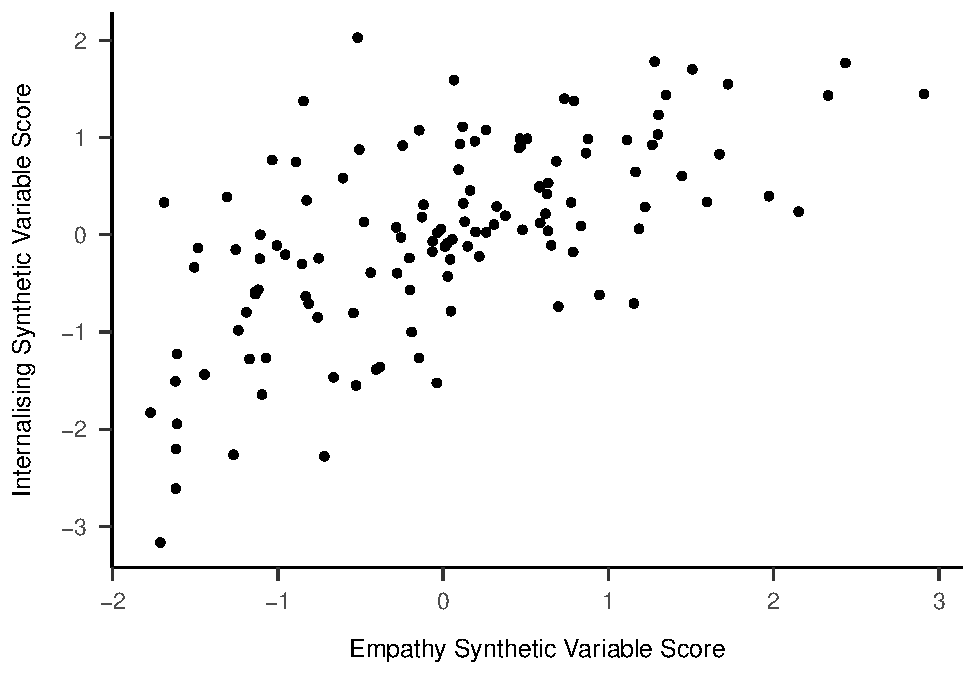
\includegraphics{papaja_cca_files/figure-latex/scatterplot-1.pdf}
\caption{\label{fig:scatterplot}Scatterplot displaying the correlation between the empathy synthetic variable
(linear combination of the original empathy measures and the covariates), and the internalizing
synthetic variable from the first function in the CCA.}
\end{figure}

\begin{table}[tbp]

\begin{center}
\begin{threeparttable}

\caption{\label{tab:coeffxtable}Coefficients for X variables, first function.}

\small{

\begin{tabular}{lccccc}
\toprule
X Variables & Standardized X canonical coefficients & Structure coefficient ($r_{s}$) & Squared structure coefficient ($r^{2}_{s}$) & Para. $p$ ($r_{s}$) & Non-para. $p$ ($r_{s}$)\\
\midrule
Affective Sharing & -0.50 & -.62 & .38 & < .001* & < .001*\\
Cognitive Empathy & 0.48 & .25 & .06 & .004 & .002*\\
Empathic Concern & 0.06 & .02 & .00 & .803 & .402\\
Empathic Distress & -0.34 & -.49 & .24 & < .001* & < .001*\\
Silent Films & -0.01 & -.02 & .00 & .812 & .411\\
Sex & -0.46 & -.60 & .36 & < .001* & < .001*\\
IQ & 0.08 & .08 & .01 & .353 & .177\\
Parent Education & -0.09 & -.02 & .00 & .841 & .411\\
Neighborhood Advantage & 0.34 & .34 & .12 & < .001* & < .001*\\
\bottomrule
\addlinespace
\end{tabular}

}

\begin{tablenotes}[para]
\normalsize{\textit{Note.} * Survive correction for multiple comparisons (Bonferroni). Bold text = both 
          parametric and non-parametric p-value significant.}
\end{tablenotes}

\end{threeparttable}
\end{center}

\end{table}

\begin{table}[tbp]

\begin{center}
\begin{threeparttable}

\caption{\label{tab:coeffytable}Coefficients for Y variables, first function.}

\small{

\begin{tabular}{lccccc}
\toprule
Y Variables & Standardized Y canonical coefficients & Structure coefficient ($r_{s}$) & Squared structure coefficient ($r^{2}_{s}$) & Para. $p$ ($r_{s}$) & Non-para. $p$ ($r_{s}$)\\
\midrule
Negative mood/physical symptoms & -0.04 & -.37 & .14 & < .001* & < .001*\\
Negative self-esteem & -0.05 & -.30 & .09 & .001* & < .001*\\
Ineffectiveness & -0.23 & -.46 & .22 & < .001* & < .001*\\
Interpersonal problems & 0.05 & -.30 & .09 & < .001* & < .001*\\
Separation anxiety & -0.47 & -.74 & .54 & < .001* & < .001*\\
Social phobia & -0.72 & -.86 & .74 & < .001* & < .001*\\
Physical injury fears & -0.06 & -.50 & .25 & < .001* & < .001*\\
Generalized anxiety & -0.19 & -.55 & .31 & < .001* & < .001*\\
Obsessive compulsive & 0.28 & -.36 & .13 & < .001* & < .001*\\
Panic/agoraphobia & 0.34 & -.37 & .13 & < .001* & < .001*\\
\bottomrule
\addlinespace
\end{tabular}

}

\begin{tablenotes}[para]
\normalsize{\textit{Note.} * Survive correction for multiple comparisons (Bonferroni). Bold text = both 
          parametric and non-parametric p-value significant.}
\end{tablenotes}

\end{threeparttable}
\end{center}

\end{table}

\hypertarget{supplementary-tables}{%
\section{Supplementary Tables}\label{supplementary-tables}}

\begin{table}[tbp]

\begin{center}
\begin{threeparttable}

\caption{\label{tab:tscore_table}T-scores from the CDI and SCAS measures}

\small{

\begin{tabular}{lcc}
\toprule
Internalizing scale t-score bracket & Frequency & Percentage\\
\midrule
CDI &  & \\
\ \ \ Average (40-60) & 102 & 80.31\\
\ \ \ High Average (60-65) & 12 & 9.45\\
\ \ \ Elevated (65-70) & 6 & 4.72\\
\ \ \ Very elevated (70+) & 7 & 5.51\\
SCAS &  & \\
\ \ \ Average (40-60). & 121 & 95.28\\
\ \ \ Elevated (60-65) - top 16\% of population & 2 & 1.57\\
\ \ \ (65-70) - top 6\% of population & 3 & 2.36\\
\ \ \ (70+) - top 2\% of population & 1 & 0.79\\
\bottomrule
\addlinespace
\end{tabular}

}

\begin{tablenotes}[para]
\normalsize{\textit{Note.} T-scores have a mean of 50 and a standard deviation of 10. There were 25 children 
  (20\%) scoring higher than average depressive symptoms in the sample.  For anxiety symptoms, there 
  were only 6 children (5\%) scoring higher than average. The t-scores suggest 16\% of the population 
  in this age group might be expected to score higher than average. (For CDI see Kovacs, 2010; for 
  SCAS see https://www.scaswebsite.com/index.php?p=1\_9).}
\end{tablenotes}

\end{threeparttable}
\end{center}

\end{table}

\begin{table}[tbp]

\begin{center}
\begin{threeparttable}

\caption{\label{tab:alt1_ccatable}Pertinent values from the CCA analysis for each of the five canonical functions 
          created from alternate model one}

\small{

\begin{tabular}{lcccccccccc}
\toprule
Dim. & $R_{c}$ & $R^{2}_{c}$ & Wilk’s $\Lambda$ & Multiple $F$ & $df$ 1 & $df$ 2 & Para. $p$ ($F$) & Non-para. $p$ ($F$) & Para. $p$ ($R_{c}$) & Non-para. $p$ ($R_{c}$)\\
\midrule
1 & .57 & .32 & .34 & 1.88 & 70 & 518.27 & < .001*** & < .001*** & < .001*** & .010**\\
2 & .55 & .30 & .50 & 1.60 & 52 & 424.27 & .007** & < .001*** & < .001*** & .020*\\
3 & .43 & .18 & .72 & 1.08 & 36 & 325.73 & .351 & .007** & < .001*** & .780\\
4 & .33 & .11 & .87 & 0.70 & 22 & 222.00 & .840 & .120 & < .001*** & > .999\\
5 & .13 & .02 & .98 & 0.19 & 10 & 112.00 & .996 & .919 & .143 & > .999\\
\bottomrule
\addlinespace
\end{tabular}

}

\begin{tablenotes}[para]
\normalsize{\textit{Note.} * = <0.05, bold text = both parametric and non-parametric p-value significant. 
          Although the first and second functions were both significant, only the first function was interpreted as this was consistent across all three models (in addition the main associations within 
          the second function appear to be between the cognitive empathy task and IQ). Abbreviations: 
          Dim. = Dimension, *Rc* = Canonical Correlation, *Rc2* = Canonical Correlation Squared, 
          para. = parametric.}
\end{tablenotes}

\end{threeparttable}
\end{center}

\end{table}

\begin{table}[tbp]

\begin{center}
\begin{threeparttable}

\caption{\label{tab:alt1_coeffxtable}Coefficients for X variables, first function.}

\small{

\begin{tabular}{lccccc}
\toprule
X Variables & Standardized X canonical coefficients & Structure coefficient ($r_{s}$) & Squared structure coefficient ($r^{2}_{s}$) & Para. $p$ ($r_{s}$) & Non-para. $p$ ($r_{s}$)\\
\midrule
Affective Sharing & -0.74 & -.87 & .76 & < .001* & < .001*\\
Cognitive Empathy & 0.34 & -.03 & .00 & .779 & .389\\
Empathic Concern & -0.04 & -.25 & .06 & .005 & .002*\\
Empathic Distress & -0.47 & -.75 & .57 & < .001* & < .001*\\
Silent Films & -0.04 & -.03 & .00 & .733 & .371\\
\bottomrule
\addlinespace
\end{tabular}

}

\begin{tablenotes}[para]
\normalsize{\textit{Note.} * Survive correction for multiple comparisons (Bonferroni). Bold text = both 
          parametric and non-parametric p-value significant.}
\end{tablenotes}

\end{threeparttable}
\end{center}

\end{table}

\begin{table}[tbp]

\begin{center}
\begin{threeparttable}

\caption{\label{tab:alt1_coeffytable}Coefficients for Y variables, first function.}

\small{

\begin{tabular}{lccccc}
\toprule
Y Variables & Standardized Y canonical coefficients & Structure coefficient ($r_{s}$) & Squared structure coefficient ($r^{2}_{s}$) & Para. $p$ ($r_{s}$) & Non-para. $p$ ($r_{s}$)\\
\midrule
Negative mood/physical symptoms & -0.10 & -.38 & .15 & < .001* & < .001*\\
Negative self-esteem & 0.21 & -.06 & .00 & .494 & .252\\
Ineffectiveness & -0.24 & -.41 & .17 & < .001* & < .001*\\
Interpersonal problems & 0.04 & -.28 & .08 & .001* & < .001*\\
Separation anxiety & -0.13 & -.60 & .36 & < .001* & < .001*\\
Social phobia & -0.61 & -.86 & .75 & < .001* & < .001*\\
Physical injury fears & -0.03 & -.51 & .26 & < .001* & < .001*\\
Generalized anxiety & -0.35 & -.73 & .53 & < .001* & < .001*\\
Obsessive compulsive & 0.07 & -.49 & .24 & < .001* & < .001*\\
Panic/agoraphobia & 0.11 & -.53 & .28 & < .001* & < .001*\\
Sex & -0.17 & -.42 & .18 & < .001* & < .001*\\
IQ & -0.18 & -.19 & .03 & .036 & .018\\
Parent Education & 0.00 & -.09 & .01 & .303 & .151\\
Neighborhood Advantage & -0.14 & .01 & .00 & .919 & .454\\
\bottomrule
\addlinespace
\end{tabular}

}

\begin{tablenotes}[para]
\normalsize{\textit{Note.} * Survive correction for multiple comparisons (Bonferroni). Bold text = both 
          parametric and non-parametric p-value significant.}
\end{tablenotes}

\end{threeparttable}
\end{center}

\end{table}

\begin{table}[tbp]

\begin{center}
\begin{threeparttable}

\caption{\label{tab:alt2_ccatable}Pertinent values from the CCA analysis for each of the five canonical functions
          created from alternate model two}

\small{

\begin{tabular}{lcccccccccc}
\toprule
Dim. & $R_{c}$ & $R^{2}_{c}$ & Wilk’s $\Lambda$ & Multiple $F$ & $df$ 1 & $df$ 2 & Para. $p$ ($F$) & Non-para. $p$ ($F$) & Para. $p$ ($R_{c}$) & Non-para. $p$ ($R_{c}$)\\
\midrule
1 & .53 & .28 & .50 & 1.68 & 50 & 514.16 & .003** & .003** & < .001*** & .007**\\
2 & .49 & .24 & .69 & 1.20 & 36 & 425.20 & .199 & .019* & < .001*** & < .001***\\
3 & .26 & .07 & .91 & 0.46 & 24 & 331.24 & .988 & .803 & .003** & .459\\
4 & .15 & .02 & .98 & 0.21 & 14 & 230.00 & .999 & .964 & .097 & .892\\
5 & .05 & .00 & > .99 & 0.06 & 6 & 116.00 & .999 & .988 & .550 & .988\\
\bottomrule
\addlinespace
\end{tabular}

}

\begin{tablenotes}[para]
\normalsize{\textit{Note.} * = <0.05, bold text = both parametric and non-parametric p-value significant. 
          Abbreviations: Dim. = Dimension, *Rc* = Canonical Correlation, *Rc2* = Canonical 
          Correlation Squared, para. = parametric.}
\end{tablenotes}

\end{threeparttable}
\end{center}

\end{table}

\begin{table}[tbp]

\begin{center}
\begin{threeparttable}

\caption{\label{tab:alt2_coeffxtable}Coefficients for X variables, first function.}

\small{

\begin{tabular}{lccccc}
\toprule
X Variables & Standardized X canonical coefficients & Structure coefficient ($r_{s}$) & Squared structure coefficient ($r^{2}_{s}$) & Para. $p$ ($r_{s}$) & Non-para. $p$ ($r_{s}$)\\
\midrule
Affective Sharing & -0.74 & -.85 & .73 & < .001* & < .001*\\
Cognitive Empathy & 0.40 & .08 & .01 & .354 & .174\\
Empathic Concern & -0.04 & -.19 & .04 & .034 & .016\\
Empathic Distress & -0.41 & -.69 & .47 & < .001* & < .001*\\
Silent Films & 0.19 & .25 & .06 & .005 & .002*\\
\bottomrule
\addlinespace
\end{tabular}

}

\begin{tablenotes}[para]
\normalsize{\textit{Note.} * Survive correction for multiple comparisons (Bonferroni). Bold text = both 
          parametric and non-parametric p-value significant.}
\end{tablenotes}

\end{threeparttable}
\end{center}

\end{table}

\begin{table}[tbp]

\begin{center}
\begin{threeparttable}

\caption{\label{tab:alt2_coeffytable}Coefficients for Y variables, first function.}

\small{

\begin{tabular}{lccccc}
\toprule
Y Variables & Standardized Y canonical coefficients & Structure coefficient ($r_{s}$) & Squared structure coefficient ($r^{2}_{s}$) & Para. $p$ ($r_{s}$) & Non-para. $p$ ($r_{s}$)\\
\midrule
Negative mood/physical symptoms & -0.08 & -.37 & .14 & < .001* & < .001*\\
Negative self-esteem & 0.26 & -.01 & .00 & .919 & .451\\
Ineffectiveness & -0.22 & -.46 & .21 & < .001* & < .001*\\
Interpersonal problems & 0.08 & -.22 & .05 & .014 & .007\\
Separation anxiety & -0.17 & -.59 & .35 & < .001* & < .001*\\
Social phobia & -0.62 & -.88 & .77 & < .001* & < .001*\\
Physical injury fears & -0.09 & -.52 & .28 & < .001* & < .001*\\
Generalized anxiety & -0.36 & -.73 & .54 & < .001* & < .001*\\
Obsessive compulsive & -0.06 & -.60 & .35 & < .001* & < .001*\\
Panic/agoraphobia & 0.20 & -.55 & .30 & < .001* & < .001*\\
\bottomrule
\addlinespace
\end{tabular}

}

\begin{tablenotes}[para]
\normalsize{\textit{Note.} * Survive correction for multiple comparisons (Bonferroni). Bold text = both 
          parametric and non-parametric p-value significant.}
\end{tablenotes}

\end{threeparttable}
\end{center}

\end{table}

\newpage

\hypertarget{references}{%
\section{References}\label{references}}

\begingroup
\setlength{\parindent}{-0.5in}
\setlength{\leftskip}{0.5in}

\hypertarget{refs}{}
\leavevmode\hypertarget{ref-R-gridExtra}{}%
Auguie, B. (2017). \emph{GridExtra: Miscellaneous functions for "grid" graphics}. Retrieved from \url{https://CRAN.R-project.org/package=gridExtra}

\leavevmode\hypertarget{ref-R-papaja}{}%
Aust, F., \& Barth, M. (2020). \emph{papaja: Create APA manuscripts with R Markdown}. Retrieved from \url{https://github.com/crsh/papaja}

\leavevmode\hypertarget{ref-R-AMR}{}%
Berends, M. S., Luz, C. F., Friedrich, A. W., Sinha, B. N. M., Albers, C. J., \& Glasner, C. (2019). AMR - an r package for working with antimicrobial resistance data. \emph{bioRxiv}. Retrieved from \url{https://doi.org/10.1101/810622}

\leavevmode\hypertarget{ref-R-corx}{}%
Conigrave, J. (2020). \emph{Corx: Create and format correlation matrices}. Retrieved from \url{https://CRAN.R-project.org/package=corx}

\leavevmode\hypertarget{ref-R-car}{}%
Fox, J., \& Weisberg, S. (2019). \emph{An R companion to applied regression} (Third). Thousand Oaks CA: Sage. Retrieved from \url{https://socialsciences.mcmaster.ca/jfox/Books/Companion/}

\leavevmode\hypertarget{ref-R-carData}{}%
Fox, J., Weisberg, S., \& Price, B. (2020). \emph{CarData: Companion to applied regression data sets}. Retrieved from \url{https://CRAN.R-project.org/package=carData}

\leavevmode\hypertarget{ref-R-lubridate}{}%
Grolemund, G., \& Wickham, H. (2011). Dates and times made easy with lubridate. \emph{Journal of Statistical Software}, \emph{40}(3), 1--25. Retrieved from \url{http://www.jstatsoft.org/v40/i03/}

\leavevmode\hypertarget{ref-R-mctest_b}{}%
Imdad, M. U., Aslam, M., Altaf, S., \& Munir, A. (2019). Some new diagnostics of multicollinearity in linear regression model. \emph{Sains Malaysiana}, \emph{48(9)}, 2051--2060. Retrieved from \url{http://dx.doi.org/10.17576/jsm-2019-4809-26}

\leavevmode\hypertarget{ref-R-mctest_a}{}%
Imdadullah, M., Aslam, M., \& Altaf, S. (2016). Mctest: An r package for deteection of collinearity among regressors. \emph{The R Journal}, \emph{8(2)}, 499--509. Retrieved from \url{https://journal.r-project.org/archive/2016/RJ-2016-062/index.html}

\leavevmode\hypertarget{ref-R-ppcor}{}%
Kim, S. (2015). \emph{Ppcor: Partial and semi-partial (part) correlation}. Retrieved from \url{https://CRAN.R-project.org/package=ppcor}

\leavevmode\hypertarget{ref-R-jtools}{}%
Long, J. A. (2020). \emph{Jtools: Analysis and presentation of social scientific data}. Retrieved from \url{https://cran.r-project.org/package=jtools}

\leavevmode\hypertarget{ref-R-base}{}%
R Core Team. (2020). \emph{R: A language and environment for statistical computing}. Vienna, Austria: R Foundation for Statistical Computing. Retrieved from \url{https://www.R-project.org/}

\leavevmode\hypertarget{ref-R-psych}{}%
Revelle, W. (2019). \emph{Psych: Procedures for psychological, psychometric, and personality research}. Evanston, Illinois: Northwestern University. Retrieved from \url{https://CRAN.R-project.org/package=psych}

\leavevmode\hypertarget{ref-R-numform}{}%
Rinker, T. W. (2020). \emph{numform: A publication style number and plot formatter}. Retrieved from \url{http://github.com/trinker/numform}

\leavevmode\hypertarget{ref-R-GGally}{}%
Schloerke, B., Cook, D., Larmarange, J., Briatte, F., Marbach, M., Thoen, E., \ldots{} Crowley, J. (2020). \emph{GGally: Extension to 'ggplot2'}. Retrieved from \url{https://CRAN.R-project.org/package=GGally}

\leavevmode\hypertarget{ref-R-apaTables}{}%
Stanley, D. (2018). \emph{ApaTables: Create american psychological association (apa) style tables}. Retrieved from \url{https://CRAN.R-project.org/package=apaTables}

\leavevmode\hypertarget{ref-R-MASS}{}%
Venables, W. N., \& Ripley, B. D. (2002). \emph{Modern applied statistics with s} (Fourth). New York: Springer. Retrieved from \url{http://www.stats.ox.ac.uk/pub/MASS4}

\leavevmode\hypertarget{ref-R-corrplot2017}{}%
Wei, T., \& Simko, V. (2017). \emph{R package "corrplot": Visualization of a correlation matrix}. Retrieved from \url{https://github.com/taiyun/corrplot}

\leavevmode\hypertarget{ref-R-plyr}{}%
Wickham, H. (2011). The split-apply-combine strategy for data analysis. \emph{Journal of Statistical Software}, \emph{40}(1), 1--29. Retrieved from \url{http://www.jstatsoft.org/v40/i01/}

\leavevmode\hypertarget{ref-R-ggplot2}{}%
Wickham, H. (2016). \emph{Ggplot2: Elegant graphics for data analysis}. Springer-Verlag New York. Retrieved from \url{https://ggplot2.tidyverse.org}

\leavevmode\hypertarget{ref-R-dplyr}{}%
Wickham, H., François, R., Henry, L., \& Müller, K. (2020). \emph{Dplyr: A grammar of data manipulation}. Retrieved from \url{https://CRAN.R-project.org/package=dplyr}

\endgroup

\end{document}
